\documentclass[a4paper,11pt,fleqn,twoside,notitlepage]{report}
\usepackage[]{graphicx}\usepackage[]{color}
%% maxwidth is the original width if it is less than linewidth
%% otherwise use linewidth (to make sure the graphics do not exceed the margin)
\makeatletter
\def\maxwidth{ %
  \ifdim\Gin@nat@width>\linewidth
    \linewidth
  \else
    \Gin@nat@width
  \fi
}
\makeatother

\definecolor{fgcolor}{rgb}{0.345, 0.345, 0.345}
\newcommand{\hlnum}[1]{\textcolor[rgb]{0.686,0.059,0.569}{#1}}%
\newcommand{\hlstr}[1]{\textcolor[rgb]{0.192,0.494,0.8}{#1}}%
\newcommand{\hlcom}[1]{\textcolor[rgb]{0.678,0.584,0.686}{\textit{#1}}}%
\newcommand{\hlopt}[1]{\textcolor[rgb]{0,0,0}{#1}}%
\newcommand{\hlstd}[1]{\textcolor[rgb]{0.345,0.345,0.345}{#1}}%
\newcommand{\hlkwa}[1]{\textcolor[rgb]{0.161,0.373,0.58}{\textbf{#1}}}%
\newcommand{\hlkwb}[1]{\textcolor[rgb]{0.69,0.353,0.396}{#1}}%
\newcommand{\hlkwc}[1]{\textcolor[rgb]{0.333,0.667,0.333}{#1}}%
\newcommand{\hlkwd}[1]{\textcolor[rgb]{0.737,0.353,0.396}{\textbf{#1}}}%

\usepackage{framed}
\makeatletter
\newenvironment{kframe}{%
 \def\at@end@of@kframe{}%
 \ifinner\ifhmode%
  \def\at@end@of@kframe{\end{minipage}}%
  \begin{minipage}{\columnwidth}%
 \fi\fi%
 \def\FrameCommand##1{\hskip\@totalleftmargin \hskip-\fboxsep
 \colorbox{shadecolor}{##1}\hskip-\fboxsep
     % There is no \\@totalrightmargin, so:
     \hskip-\linewidth \hskip-\@totalleftmargin \hskip\columnwidth}%
 \MakeFramed {\advance\hsize-\width
   \@totalleftmargin\z@ \linewidth\hsize
   \@setminipage}}%
 {\par\unskip\endMakeFramed%
 \at@end@of@kframe}
\makeatother

\definecolor{shadecolor}{rgb}{.97, .97, .97}
\definecolor{messagecolor}{rgb}{0, 0, 0}
\definecolor{warningcolor}{rgb}{1, 0, 1}
\definecolor{errorcolor}{rgb}{1, 0, 0}
\newenvironment{knitrout}{}{} % an empty environment to be redefined in TeX

\usepackage{alltt}
\newcommand{\SweaveOpts}[1]{}  % do not interfere with LaTeX
\newcommand{\SweaveInput}[1]{} % because they are not real TeX commands
\newcommand{\Sexpr}[1]{}       % will only be parsed by R


\usepackage[utf8]{inputenc}
\usepackage[margin=2.5cm]{geometry}
\usepackage{graphicx}
\usepackage[T1]{fontenc}
\usepackage{amsmath}

\usepackage{csquotes}
\usepackage[english]{babel}
\usepackage{float}
\usepackage{caption}
\usepackage{makecell}
\usepackage{hyperref}
\usepackage{bm}
\usepackage{newfloat}
\usepackage{amsfonts}

\usepackage[linesnumbered,lined,boxed,commentsnumbered]{algorithm2e}

\usepackage{tikz}
%\usetikzlibrary{calc,trees,positioning,arrows,chains,shapes.geometric,%
%    decorations.pathreplacing,decorations.pathmorphing,shapes,%
%    matrix,shapes.symbols}

% \tikzstyle{punktchain} = [rectangle,
%     rounded corners,
%     draw=black, very thick,
%     text width=10em,
%     minimum height=3em,
%     text centered,
%     on chain,
%     top color=white,
%     bottom color=blue!20]
    
%\tikzset{arrow} = [thick,->,>=stealth]
\usepackage{fancyhdr}
\setlength{\headheight}{15pt}

\pagestyle{fancy}
\renewcommand{\chaptermark}[1]{ \markboth{#1}{} }
\renewcommand{\sectionmark}[1]{ \markright{#1}{} }

\fancyhf{}
\fancyfoot[CE,CO]{\thepage}
\fancyhead[LE]{\textit{ \nouppercase{\leftmark}} }
\fancyhead[LO]{\textit{ \nouppercase{\rightmark}} }
%\fancyhead[RE,RO]{Erik Thors\'{e}n, \href{mailto:Ethorsn@gmail.com}{Ethorsn@gmail.com} }
\fancypagestyle{plain}{ %
\fancyhf{} % remove everything
  \renewcommand{\headrulewidth}{0pt} % remove lines as well
  \renewcommand{\footrulewidth}{0pt}
}

\usepackage[
citestyle=authoryear,
bibstyle=authoryear,
backend=bibtex
]{biblatex}

\addbibresource{REFERENCES.bib}
\title{Quality control in next-generation sequencing quality control data?}
\author{Erik Thors\'{e}n \thanks{Postal adress: Mathematical Statistics, Stockholm University, SE-106 91, Sweden. E-mail: Ethorsn@gmail.com. Supervisor: Taras Bodnar and Johan Dahlberg}}
\date{\today}

\raggedbottom


\begin{document}



As previously described, it is not possible to observe the machines under what could be deemed as in control behaviour. The parameters of interest need to be estimated from the data. Before doing so, we transform the data, using the following box-cox transformation, presented in \cite{BoxCox}, 
$$
Y=
\begin{cases}
\frac{Y^{\lambda}-1}{\lambda} & \text{for } \lambda \neq 0 \\
\log(Y) & \text{else}.
\end{cases}
$$
The data are transformed independently. The parameter $\lambda$ is estimated using the method suggested in \cite{Gurrero}. Both the box cox transformation and the guerro estimation method is implemented in the \texttt{forecast} package. No more attention will be put into these methods. 

Two statistical tests of the normal assumption are presented in Table \ref{TestTable}, performed on the transformed data. Henze-Zirkler's multivariate test of normality, presented in \cite{HenzeZirkler}, shows some evidence against the null that data is not normally distributed. The genaralized Shapiro-Wilk test of normality, presented in \cite{GenShapWilk}, shows no evidence at all.
% latex table generated in R 3.2.3 by xtable 1.8-2 package
% Fri May 20 16:07:59 2016
\begin{table}[ht]
\centering
\begin{tabular}{rlr}
  \hline
 & Test & P.value \\ 
  \hline
1 & Henze-Zirkler's & 0.22 \\ 
  2 & Generalized Shapiro-Wilk & 0.00 \\ 
   \hline
\end{tabular}
\caption{Two statistical tests of normality, Henze-Zirkler's and a generalized Shapiro-Wilk's test. One out of two tests approves of the normality assumption.} 
\label{TestTable}
\end{table}

Under the assumption that data \textit{is} normally transformed, the autocorrelation may be investigated. If the autocorrelation at a given lag is below the standard normal distributions $95\%$ percentile we can assume that the data is independent in time. There are a total of 1128 correlation coefficients to investigate. We will show the proportion of lags which are greater than the standard normal distributions $95\%$ percentile and all autocorrelation coefficients, for a given lag, in a histogram. 
For the HiSeq 6 machine, the proportion of autocorrelation coefficients greater than the normal quantile are seen in Table \ref{ACFtable} for lags one through five. Under the assumption of normally distributed data, it can be seen that the HiSeq 6 data does not seem to be independent in time. However, since the transformed data shows little evidence that it is normally disitributed, any conclusions on the independence between observations in a temporal manner, could be highly inapproriate and inaccurate. The autocorrelation for the first two lags are shown in Figure \ref{fig:FigureACF}. 

We can also test the assumption that the estimated covariance matrix is a positive definite matrix using the \texttt{is.positive.definite} function from the \texttt{matrixcalc} package. 

The result from the function is $TRUE$, the estimated covariance matrix is positive definite. 

\begin{kframe}
\begin{alltt}
\hlkwd{library}\hlstd{(dplyr)}
\end{alltt}


{\ttfamily\noindent\itshape\color{messagecolor}{\#\# \\\#\# Attaching package: 'dplyr'}}

{\ttfamily\noindent\itshape\color{messagecolor}{\#\# The following objects are masked from 'package:stats':\\\#\# \\\#\#\ \ \ \  filter, lag}}

{\ttfamily\noindent\itshape\color{messagecolor}{\#\# The following objects are masked from 'package:base':\\\#\# \\\#\#\ \ \ \  intersect, setdiff, setequal, union}}\begin{alltt}
\hlkwd{library}\hlstd{(ggplot2)}
\hlstd{CalculatePropACF} \hlkwb{<-} \hlkwa{function}\hlstd{(}\hlkwc{x}\hlstd{,}\hlkwc{lag}\hlstd{)\{}

  \hlstd{tmp.strings} \hlkwb{<-} \hlkwd{colnames}\hlstd{(x)}

  \hlstd{x.tmp} \hlkwb{<-} \hlstd{x[,}\hlkwd{order}\hlstd{(tmp.strings)]}

  \hlstd{ACF} \hlkwb{<-} \hlkwd{acf}\hlstd{(x.tmp,} \hlkwc{plot}\hlstd{=}\hlnum{FALSE}\hlstd{,} \hlkwc{lag.max}\hlstd{=lag)}

  \hlcom{# allocate matrix}
  \hlstd{tmp} \hlkwb{<-} \hlkwd{matrix}\hlstd{(}\hlkwc{ncol}\hlstd{=}\hlkwd{dim}\hlstd{(ACF}\hlopt{$}\hlstd{acf)[}\hlnum{2}\hlstd{],}\hlkwc{nrow}\hlstd{=}\hlkwd{dim}\hlstd{(ACF}\hlopt{$}\hlstd{acf)[}\hlnum{3}\hlstd{])}
  \hlcom{# extract the lag which is supposed to be investigated}
  \hlkwa{for} \hlstd{(i} \hlkwa{in} \hlnum{1}\hlopt{:}\hlkwd{dim}\hlstd{(ACF}\hlopt{$}\hlstd{acf)[}\hlnum{3}\hlstd{])\{}
    \hlcom{# the first element of $acf is equal to the correlation therefore lag+1.}
    \hlstd{tmp[i,]} \hlkwb{<-} \hlstd{ACF}\hlopt{$}\hlstd{acf[lag}\hlopt{+}\hlnum{1}\hlstd{,,i]}
  \hlstd{\}}
  \hlcom{#normal quantile}
  \hlstd{limit} \hlkwb{<-} \hlnum{1.96}\hlopt{/}\hlkwd{sqrt}\hlstd{(ACF}\hlopt{$}\hlstd{n.used)}

  \hlstd{nom} \hlkwb{<-} \hlkwd{which}\hlstd{(}\hlkwd{abs}\hlstd{(tmp[}\hlkwd{upper.tri}\hlstd{(tmp,} \hlkwc{diag}\hlstd{=}\hlnum{TRUE}\hlstd{)])}\hlopt{>}\hlstd{limit)}

  \hlstd{denom} \hlkwb{<-} \hlstd{tmp[}\hlkwd{upper.tri}\hlstd{(tmp,} \hlkwc{diag}\hlstd{=}\hlnum{TRUE}\hlstd{)]} \hlopt \hlstd{length}

  \hlstd{prop} \hlkwb{<-} \hlkwd{length}\hlstd{(nom)}\hlopt{/}\hlstd{denom}
  \hlkwd{return}\hlstd{(}\hlkwd{list}\hlstd{(}\hlstr{"Props"}\hlstd{=prop,}
              \hlstr{"AutoCorr"}\hlstd{=tmp[}\hlkwd{upper.tri}\hlstd{(tmp,} \hlkwc{diag}\hlstd{=}\hlnum{TRUE}\hlstd{)]}
  \hlstd{))}
\hlstd{\}}
\hlstd{propList} \hlkwb{<-} \hlkwd{lapply}\hlstd{(}\hlnum{1}\hlopt{:}\hlnum{5}\hlstd{,}\hlkwa{function}\hlstd{(}\hlkwc{x}\hlstd{)} \hlkwd{CalculatePropACF}\hlstd{(TransformedData,x))}

\hlstd{Proportions} \hlkwb{<-} \hlkwd{lapply}\hlstd{(}\hlnum{1}\hlopt{:}\hlkwd{length}\hlstd{(propList),} \hlkwa{function}\hlstd{(}\hlkwc{x}\hlstd{) propList[[x]]}\hlopt{$}\hlstd{Props)} \hlopt \hlkwd{unlist}\hlstd{()}
\hlstd{AutoCorr} \hlkwb{<-} \hlkwd{lapply}\hlstd{(}\hlnum{1}\hlopt{:}\hlkwd{length}\hlstd{(propList),} \hlkwa{function}\hlstd{(}\hlkwc{x}\hlstd{) propList[[x]]}\hlopt{$}\hlstd{AutoCorr)}

\hlstd{x.tabl} \hlkwb{<-} \hlstd{xtable}\hlopt{::}\hlkwd{xtable}\hlstd{(}\hlkwd{data.frame}\hlstd{(}\hlkwc{Lag}\hlstd{=}\hlnum{1}\hlopt{:}\hlnum{5}\hlstd{,}\hlkwc{Proportion}\hlstd{=Proportions),} \hlkwc{caption}\hlstd{=}\hlstr{"Proportion of autocorrelation greater than the normal 95 percentile, at lags 1 through 5."}\hlstd{,} \hlkwc{label}\hlstd{=}\hlstr{"ACFtable"}\hlstd{)}
\hlkwd{print.xtable}\hlstd{(x.tabl,}\hlkwc{include.rownames} \hlstd{=} \hlnum{FALSE}\hlstd{)}
\end{alltt}
\end{kframe}% latex table generated in R 3.2.3 by xtable 1.8-2 package
% Fri May 20 16:07:59 2016
\begin{table}[ht]
\centering
\begin{tabular}{rr}
  \hline
Lag & Proportion \\ 
  \hline
  1 & 0.24 \\ 
    2 & 0.10 \\ 
    3 & 0.05 \\ 
    4 & 0.04 \\ 
    5 & 0.05 \\ 
   \hline
\end{tabular}
\caption{Proportion of autocorrelation greater than the normal 95 percentile, at lags 1 through 5.} 
\label{ACFtable}
\end{table}
\begin{kframe}\begin{alltt}
\hlkwd{library}\hlstd{(gridExtra)}

\hlstd{p1}\hlkwb{<-} \hlkwd{ggplot}\hlstd{(}\hlkwd{data.frame}\hlstd{(}\hlkwc{x}\hlstd{=AutoCorr[[}\hlnum{1}\hlstd{]]))} \hlopt{+}
  \hlkwd{geom_histogram}\hlstd{(}\hlkwd{aes}\hlstd{(}\hlkwc{x}\hlstd{=x))} \hlopt{+}
  \hlkwd{theme_bw}\hlstd{()} \hlopt{+}
  \hlkwd{xlab}\hlstd{(}\hlstr{"value"}\hlstd{)} \hlopt{+}
  \hlkwd{ggtitle}\hlstd{(}\hlstr{"Autocorrelation, lag 1"}\hlstd{)}
\hlstd{p2} \hlkwb{<-} \hlkwd{ggplot}\hlstd{(}\hlkwd{data.frame}\hlstd{(}\hlkwc{x}\hlstd{=AutoCorr[[}\hlnum{2}\hlstd{]]))} \hlopt{+}
  \hlkwd{geom_histogram}\hlstd{(}\hlkwd{aes}\hlstd{(}\hlkwc{x}\hlstd{=x))} \hlopt{+}
  \hlkwd{theme_bw}\hlstd{()} \hlopt{+}
  \hlkwd{xlab}\hlstd{(}\hlstr{"value"}\hlstd{)} \hlopt{+}
  \hlkwd{ggtitle}\hlstd{(}\hlstr{"Autocorrelation, lag 2"}\hlstd{)}
\end{alltt}
\end{kframe}
\begin{center}
\begin{knitrout}
\definecolor{shadecolor}{rgb}{0.969, 0.969, 0.969}\color{fgcolor}\begin{kframe}
\begin{alltt}
\hlkwd{grid.arrange}\hlstd{(p1,p2,} \hlkwc{ncol}\hlstd{=}\hlnum{2}\hlstd{)}
\end{alltt}


{\ttfamily\noindent\itshape\color{messagecolor}{\#\# `stat\_bin()` using `bins = 30`. Pick better value with `binwidth`.\\\#\# `stat\_bin()` using `bins = 30`. Pick better value with `binwidth`.}}\end{kframe}\begin{figure}
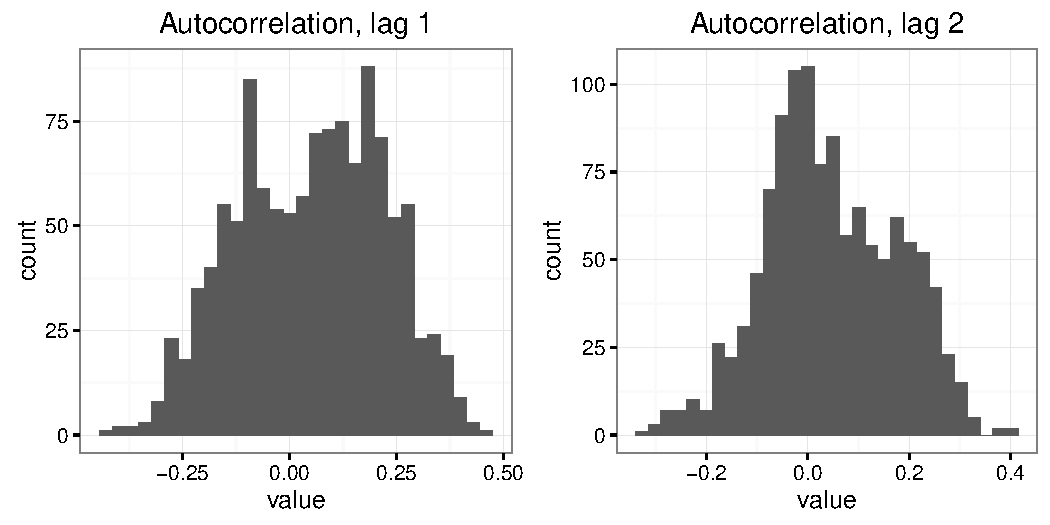
\includegraphics[width=\maxwidth]{figure/FigureACF-1} \caption[Distribution of autocorrelation coefficients at lag 1 (left) and lag 2 (right) of the transformed data]{Distribution of autocorrelation coefficients at lag 1 (left) and lag 2 (right) of the transformed data. The marked red line represents the normal 95 percentile.}\label{fig:FigureACF}
\end{figure}


\end{knitrout}
\end{center}
\end{document}
